\documentclass[a4paper]{article}
\usepackage{graphicx} % to include graphicx elements
\usepackage{tabu} % to use tables
\usepackage{geometry} % to define page layout
\usepackage[pdftex, colorlinks]{hyperref} % to use href

%----- Define page layout -----
 \geometry{
 left=25mm,
 right=25mm,
 top=30mm,
 bottom=25mm,
 headsep=7mm}
 
% -----------------------------
\begin{document}

%TITLE PAGE
\begin{titlepage}

\title{
	
\includegraphics[scale=0.5]{Images/PolimiLogo}
	\\
	\normalsize{Politecnico di Milano}\\
	{AY 2017/2018}
	\bigskip\\
	\resizebox{\linewidth}{!}{~Travlendar\textsuperscript{+}}
	\bigskip\\
	\LARGE{Requirement Analysis and Specification Document}
	\vfill
}

	\date{November 25, 2017}

\author{
	Mirko Salaris,
	Piervincenzo Ventrella,
	Pietro Cassarino
}

\maketitle
\thispagestyle{empty}

\end{titlepage}

%Define deliverable specific info
%Replace cell contents where needed
\begin{table}[h!]
\begin{tabu} to \textwidth { X[0.3,r,p] X[0.7,l,p] }
\hline
\smallskip & \smallskip\\
\textbf{Deliverable:} & RASD\\
\textbf{Title:} & Requirement Analysis and Verification Document \\
\textbf{Authors:} & Mirko Salaris, Piervincenzo Ventrella, Pietro Cassarino \\
\textbf{Version:} & 1.0 \\ 
\textbf{Date:} & 27-October-2017 \\
\textbf{Download page:} & https://github.com/mirkosalaris/CassarinoSalarisVentrella/\\
\textbf{Copyright:} & Copyright © 2017, M. Salaris, P. Ventrella, P. Cassarino\\
\hfill & All rights reserved \\
\smallskip & \smallskip\\
\hline
\end{tabu}
\end{table}

%------------------------------------------------------------------------------------------------------------------------------------------------
\newpage
\renewcommand{\contentsname}{Table of Contents} % rename from "Contents" to "Table of Contents"
{\hypersetup{hidelinks} % avoid coloring table of contents
\tableofcontents
}

\newpage
\addcontentsline{toc}{section}{List of Figures}
\listoffigures
\addcontentsline{toc}{section}{List of Tables}
\listoftables

%------------------------------------------------------------------------------------------------------------------------------------------------
\clearpage
\section{Introduction}
\label{sect:introduction}
\subsection{Purpose}
This document is the Requirement Analysis and Specification Document for the Travlendar+ application. Its aim is
to inform about what the application offers, about requirements and goals that the system must present. This document offers also an analysis of the world and of the shared phenomena regarding Travlendar+. RASD contains class diagram to show domain model and other diagrams which illustrate, with more details, transactions of the functionality of the application.
\subsection{Scope}
Travlendar+ is an application that allows people to organize and to track their appointments and meeting by 
registering them into the application. A person becomes a User of Travlendar+ by registering himself to the app. After this phase, users can start to use basic functionalities of the app (e.g. register appointments and organize meetings).\newline 
The app allows users to create appointments, eventually inviting other users of the app, facilitating communication issues.
The goal of Travlendar+ is to organize in the best way all daily commitments of its users considering all the possible problems that can influence travels and trips (e.g. weather conditions, strikes, etc.).\newline
When a User creates an event, he can add, for the travel, eventual passengers or baggage, so that the app can suggest better trip choices. Travlendar+ allows users to visualize their planned schedule too.\newline 
The dynamicity of the software allows users to set some personal preferences, for example, to set a flexible break window time for having free time or lunch, to choose eco-friendly solutions for his trips, to deactivate some transportation means.\newline 
The system interfaces with other firms (e.g. transportation companies, territory maps companies, sharing transportation companies) to offer a more comprehensive user experience. In this way, a User has the possibility to buy tickets and passes for transportation means. Moreover, the system offers a location service for vehicles of affiliated shared transport companies but to proceed with the renting the User is redirected to the company's app.

\subsubsection{Goals}
The system should:
	\begin{enumerate}[label={[G\arabic*]}]
		\item \label{G_dev_language} allow a Person to use the app in his/her device language, if the language is one of the \defined{supported languages}, English otherwise
		\item \label{G_become_registered} allow a Person to become a registered User after providing credentials
		\item \label{G_log_in} allow a Person to log in
		\item \label{G_welcome_page} allow a new User to access the welcome page
		\item \label{G_add_credit_card} allow User to add credit card data
		\item \label{G_add_licence} allow User to add driving license
		\item \label{G_pers_preferences} allow a User to set personal preferences:
		\begin{enumerate}[label=\theenumi\#{\arabic*}]
			\item \label{G_eco_friendly} specify his/her preference for eco-friendly solution
			\item \label{G_break_windows} set break time windows, either flexible or fixed
			\item \label{G_time_slot} set time slot in which the use of specific transportation means should be avoided
			\item \label{G_min_distance} set a minimum distance below which a specific transportation mean should be avoided
			\item \label{G_max_distance} set a maximum distance beyond which a specific transportation mean should be avoided
			\item \label{G_transp_disabled} set a specific transportation mean as permanently disabled
		\end{enumerate}
		\item \label{G_new_appointment} allow User to create a new appointment, specifying its details
		\item \label{G_visualize&update} allow User to visualize his/her appointments, eventually updating its details
		\item \label{G_choose_sug} during the specification of details of an appointment, allow User to visualize suggested travel solutions and to choose one of them
		\item \label{G_change_preferred_transp} during the specification of details of an appointment, before the choice, allow User to set a preferred transportation mean
		\item \label{G_invite} during the specification of details of an appointment, allow User to invite other persons to the appointment
		\item \label{G_owns_ticket} during the specification of details of an appointment, if for the selected travel solution a ticket is expected, allow User to specify if he/she owns a ticket, either ordinary or a pass (eventually specifying the deadline)
		\begin{enumerate}[label=\theenumi\#{\arabic*}]
			\item \label{G_buy_ticket} if the user does not own a ticket and the transportation company is \defined{affiliated} with Travlendar+, he/she can buy it
		\end{enumerate}
		\item \label{G_visualize_schedule} allow User to visualize daily/weekly schedule
		\item \label{G_delete} allow User to delete an existing appointment
		\item \label{G_locate} allow User to locate nearest vehicle of a vehicle sharing system, if that is the transportation mean of choice of an incoming appointment
		\item \label{G_redirection} allow User to being redirected to the company's app to proceed with the renting of the selected shared vehicle
		\item \label{G_show_suggestions} show suggestions based on: traffic, weather conditions/forecast, strikes, type of appointment, baggage, passengers
		\item \label{G_notify} notify the User about incoming appointments
		\begin{enumerate}[label=\theenumi\#{\arabic*}]
			\item \label{G_confirmation} asking for confirmation on the transportation means previously planned
			\item \label{G_notify_suggestions} in case no transportation mean was selected, suggesting one
%			\item \label{G_complications} communicating eventually complications (bad weather, traffic) and suggesting more feasible solutions
		\end{enumerate}
	\end{enumerate}

\subsection{Definitions, Acronyms, Abbreviations}
	\subsubsection{Definitions}
		\begin{description}
			% TODO Sort alphabetically
			\item[- \textit{welcome page}:] after completing the sign up process,when the user logs in for the first time, he is redirected to this page where sequentially the app asks him to insert credit-card data, driving licence data and set his preferences the user can skip any of this phases and complete them in a second time. After this process, the initial settings configuration is completed
			\item[- \textit{personal preferences}:] with this term we mean that here the user can:\newline
			- specify break time windows; \newline
			- specify the interest or not for eco-friendly solutions;\newline
			- specify constraints, such as avoiding  bike, on the travel means solutions).
			\item[- \textit{supported languages}:]
			\item[- \textit{valid credentials}:]
			\item[- \textit{appointment details}:]
			\item[- \textit{incoming appointment}:]
			\item[- \textit{affiliated company}:]
		\end{description}
	\subsubsection{Acronyms}
		\begin{description}
		\item[- \textit{S2B}:] System to Be;
		\item[- \textit{API}:] Application Programming Interface.
	\end{description}
	\subsubsection{Abbreviations}
\subsection{Revision history}
\subsection{Document Structure}

%------------------------------------------------------------------------------------------------------------------------------------------------
\clearpage
\section{Overall Description}
\label{sect:overview}
\subsection{Product perspective}
\subsection{Product functions}
\textit{TODO: here will be included a description}
	\subsubsection{Scenario 1}
	Mario is the director of his company and he has seen an ad of Travlendar+, so he wants to try it to organize the weekly meetings with his employees. After the installation, he has to register to the app. The first thing he creates is his weekly program. We work from Monday to Friday, from 8 am to 16 pm.\newline
	There is an actual meeting coming up on Friday at 8 pm, so he creates a new	meeting in the app. After setting the time and the day, he invites his employees to join the meeting. He will remain in his office, so he will not need to use	any travel means.\newline
	Giovanni is one of Mario's employee and he is registered to Travlendar+. He receives a notification and accepts the invitation to the meeting. He chooses to reach the location by walk because he will already be nearby.\newline
	Alex is another employee and does not have an account on Travlendar. He receives an email with an invitation link to register to the app. After the registration, the app redirects him to the meeting's invitation and he will proceed by accepting it and choosing to go by car. Then he explores the app and decides to add his weekly program. The app finds out that he will be in the café near the metro at 6:40 pm, so it suggests Alex to take the metro instead of the car. He accepts the suggestion.
	\subsubsection{Scenario 2}
	Paolo, a resident of Bergamo, has recently registered to Travlendar+ and during	the initial setup has specified a flexible launch break from 11:00 am to 13:00 am, with at least 40 minutes of break.\newline
	Tomorrow he is going to have an audition at 12:30 pm, in Monza. He inserts the event in the app and after having specified that the audition will end at about 13:30pm, he looks at the suggestions of the app on the travel means to take: the app suggests him some travel solutions, but he does not specify which he's going to take because he wants to think about it overnight.\newline
	The next morning, the app sends Paolo a reminder with two travel solutions:\\
	\indent- go by car, leaving at about 11.45am, arriving at 12.27 pm;\\
	\indent - take the bus, passing at 10:49 am and arriving at 11:38 am.
	\newline He chooses the second option to avoid being late at the audition.
	\subsubsection{Scenario 3}
	Alex is a professor of Bologna University, he has a short memory and is very badly organized, so he decides to rely on Travlendar+. Alex downloads it on occasion of a work trip. He signs up and decides to insert his credit card data for an eventual purchase from the app.\newline
	He needs to reach the University of Parma to hold a conference. Alex sets up the app to arrive in Parma by train. Travlendar+ asks Alex the kind of event and he specifies it is a formal work meeting. The app asks him which transport means he wants to take in order to get to the university from the railway station. Alex opts to go by bicycle, although the app suggest not to, because of the formal type of meeting.\newline
	The departure day Alex is in a shopping center with his family, he has completely forgotten that he has a train to take, but Travlendar+ solves the problem by notifying him of the appointment. At that point, Alex has no more time and chooses to buy the train tickets using the app. While he is on the train, Travlendar+ suggests him to choose another transport means (instead of a bike) because of the bad weather conditions. Alex accepts the advice and decides to take a bus.
	\subsubsection{Scenario 4}
	Luca is a meteorologist who works for a laboratory in Venice. He knows very well all the climatic problem that humans are creating in their Country. Luca finds Travlendar+ very appropriate to help in solving this problematic. He likes to opt for an Eco-friendly solution by setting up this preference in the app settings. In this way he can avoid, at least in this aspect, further damaging the environment. His favorite functionality is bike sharing because of its innovative localization system and its low environmental impact.
	\subsubsection{Scenario 5}
	\textit{Mark, son of Lucas, asks to his father to bring him  to the basketball tournament of Sunday morning.\newline
		Lucas checks the daily schedule for Sunday and he notices he already has an appointment with the hairdresser but, of course, spending time with his son is more important, so he decides to delete the previous event on the agenda and set a new one.\newline
		Mark asks to the father if also his team mate Mike can come.
		Of course Mark and Mike have to bring with them the bags with the jersey and the basketball shoes, so Lucas, creating the event on Travlendar+, after specifying the location of the basketball court, specifies also that he will bring with him baggage and passengers.\newline
		Unfortunately his car is broken, so Lucas use  the app to look for alternative solutions.\newline
		Travlendar+, taking into account the constraints previously settled by the man, suggests to him to use Enjoy or SmartToGo, two well known car sharing companies that will solve his problem.\newline
		Lucas accepts the suggested solution and proceeds with the creation of the event.
	}
	\subsubsection{Scenario 6}
	\textit{Mary, John's wife, one week ago, asked to her husband to pick the children up to school on Monday at 13.00 and, because she knows John,  forced him to take note of that with Travlendar+.\newline
		So John planned this event on the app specifying that he will use the car to do it.
		He specified also the location of the school.\newline
		On Monday morning, as usual, Travlndar+ shows to John his daily program reminding him about his children and showing the previous  travel mean planned.\newline
		John, still intentioned to pick the children up with the car, does not modify the plan, closes the app and goes to work in the other side of Milan.\newline
		At 12.00 Travlendar+, according to the GPS position of the man, suggests him to leave in 15 minutes.
		Travel+ also suggests to avoid to go through  Viale Gioia because of the traffic and take the SS1.\newline
		Thanks to Travlendar+ John manages to be on time, collect the children and make his wife proud of him. 
	}
\subsection{User characteristics}
\subsection{Assumptions, dependencies and constraints}

%------------------------------------------------------------------------------------------------------------------------------------------------
\clearpage
\section{Specific Requirements}
\label{sect:requirements}
\subsection{External Interface Requirements}
	\subsubsection{User Interfaces}
	\subsubsection{Hardware Interfaces}
	\subsubsection{Software Interfaces}
	\subsubsection{Communication Interfaces}
\subsection{UML modeling}
	\subsubsection{Use Case diagram}
		\textbf{Diagram} \\
		\indent\textit{TODO: here an image will be attached}
		\newline
		\renewcommand{\arraystretch}{1.6} % increase line height
		
		\medskip %leave a bit of space before the next 'section'
		\vbox{ % to avoid page breaking
			\noindent
			\textbf{User creates event}
			\medskip\\
			\begin{tabu} to \textwidth {| X[\fcWidth,r,p] | X[1-\fcWidth,l,p] |}
				\hline\textbf{Use case:} & User creates an event
				\\
				\hline\textbf{Actors:} & User
				\\
				\hline\textbf{Entry condition:} & The user must be logged
				\\
				\hline\textbf{Flow of events:} & The user creates an event (a meeting, appointment or generic event) giving it a name;\newline
				User specifies the location of the event;\newline
				User specifies details such as passengers or baggage;\newline
				User selects a travel mean taking to account app’s suggestion;\newline
				The app takes note of the settings and send a confirmation;\newline
				The app redirects the user to the main page.
				\\
				\hline\textbf{Secondary flows:} & User does not specify a travel mean and let it blank;\newline
				The app takes anyway note of the setting and alert the user of the missing information; \newline
				The app redirects the user to the main page.
				\\
				\hline\textbf{Exceptions:} & Warnings messages are created in the following cases:
				\begin{itemize}
					\item User creates an event that overlaps another event;
					\item User creates an event with a location that is unreachable in the allocated time;
					\item User creates an event that violates the set constraints about the break windows.
				\end{itemize}
				\\
				\hline\textbf{Post conditions:} & The user is successfully redirected to the main page.
				\\
				\hline
			\end{tabu}
			\bigskip %leave a bit of space after the table
		}
		
		\vbox{ % to avoid page breaking
			\noindent
			\textbf{Sign Up}
			\medskip\\
			\begin{tabu} to \textwidth {| X[\fcWidth,r,p] | X[1-\fcWidth,l,p] |}
				\hline\textbf{Use case:} & Sign Up
				\\
				\hline\textbf{Actors:} & Person
				\\
				\hline\textbf{Entry condition:} &user must be not already logged;
				\\
				\hline\textbf{Flow of events:} & the person inserts full name and email contact;\newline
				the app send an email with the confirmation link;\newline
				the person give the confirmation trough the link on the mail;\newline
				the app give the welcome to the new user.
				
				\\
				\hline\textbf{Secondary flows:} & none.
				\\
				\hline\textbf{Exceptions:} &the person inserts a wrong email contact;\newline
				the sign up cannot proceed.
				
				\\
				\hline\textbf{Post conditions:} & the person is successfully signed up and become an actual logged user.
				\\
				\hline
			\end{tabu}
			\bigskip %leave a bit of space after the table
		}
		
		\vbox{ % to avoid page breaking
			\noindent
			\textbf{Initial settings configuration}
			\medskip\\
			\begin{tabu} to \textwidth {| X[\fcWidth,r,p] | X[1-\fcWidth,l,p] |}
				\hline\textbf{Use case:} & Initial settings configuration
				\\
				\hline\textbf{Actors:} & User
				\\
				\hline\textbf{Entry condition:} & the User just has just completed the sign up process;\newline
				user must be logged.
				
				\\
				\hline\textbf{Flow of events:} & User insert sequentially the following  information:
				\begin{itemize}
				\item 	Credit card;
				\item 	Driving licence;
				\item 	Break time windows;
				\item	Interest for Eco-friendly solutions on the travel means.
				\item	Constraints on travel means.
				\end{itemize}
				The app, for each step,  check the info and send a confirmation;
				The app redirects the user to the main page.
				
				\\
				\hline\textbf{Secondary flows:} & User skips to specify one or more information that could be specified later in the settings.\newline
				The app notifies the user about the missing information and redirects anyway the user to the main page.
				
				\\
				\hline\textbf{Exceptions:} & user inserts inconsistent information (incorrect credid-card/licence information, break time shorter than 30 minutes);\newline
				The app allerts the user and asks him to insert again the info.
				\\
				\hline\textbf{Post conditions:} & the set configurations are successfully saved and the user is redirected to the main page.
				\\
				\hline
			\end{tabu}
			\bigskip %leave a bit of space after the table
		}
		
		\vbox{ % to avoid page breaking
			\noindent
			\textbf{User visualizes the appointment}
			\medskip\\
			\begin{tabu} to \textwidth {| X[\fcWidth,r,p] | X[1-\fcWidth,l,p] |}
				\hline\textbf{Use case:} & User visualizes the appointment.
				\\
				\hline\textbf{Actors:} & User
				\\
				\hline\textbf{Entry condition:} & user must be logged;\newline
				the event must exist;
				
				\\
				\hline\textbf{Description:} & user visualize an appointment and eventually:
				\begin{itemize}
					\item If not specified yet, set a travel mean;
					\item Modify the previous travel mean or other detail such as location, baggage or passengers;
					\item Buy a ticket for the travel mean;
					\item Rent a shared vehicle if is the proper time to do that and locate the nearest one;
					\item Delete the appointment. 
				\end{itemize}\\
				\hline
			\end{tabu}\\
			\bigskip %leave a bit of space after the table
		}
		
		\vbox{ % to avoid page breaking
			\noindent
			\textbf{User buy travel ticket}
			\medskip\\
			\begin{tabu} to \textwidth {| X[\fcWidth,r,p] | X[1-\fcWidth,l,p] |}
				\hline\textbf{Use case:} & User buy travel ticket
				\\
				\hline\textbf{Actors:} & User
				\\
				\hline\textbf{Entry condition:} & user must be logged; \newline
				user must have added a payment card .
				
				\\
				\hline\textbf{Flow of events:} &User select an event;\newline
				User,  through the app, searches for tickets for the specified travel mean; \newline
				User select the ticket’s option and picks one;\newline
				User proceeds with the payment;\newline
				The payment operation ends successfully;\newline
				The app send a confirmation and redirects the user to the main page;
				
				\\
				\hline\textbf{Secondary flows:} & none
				\\
				\hline\textbf{Exceptions:} & The payment is rejected (not enough credit, expired card, ..);\newline
				The app notifies the user; \newline
				The app redirect the user to the home page;
				
				\\
				\hline\textbf{Post conditions:} & User successfully books the tickets and is redirected to the main page.
				\\
				\hline
			\end{tabu}
		}
	\subsubsection{Class diagram}
		% don't really know what happens here, but it is fine graphically
		% ((I'm referring to '\paperwidth-1')
		\begin{figure}[H]
			\centerline{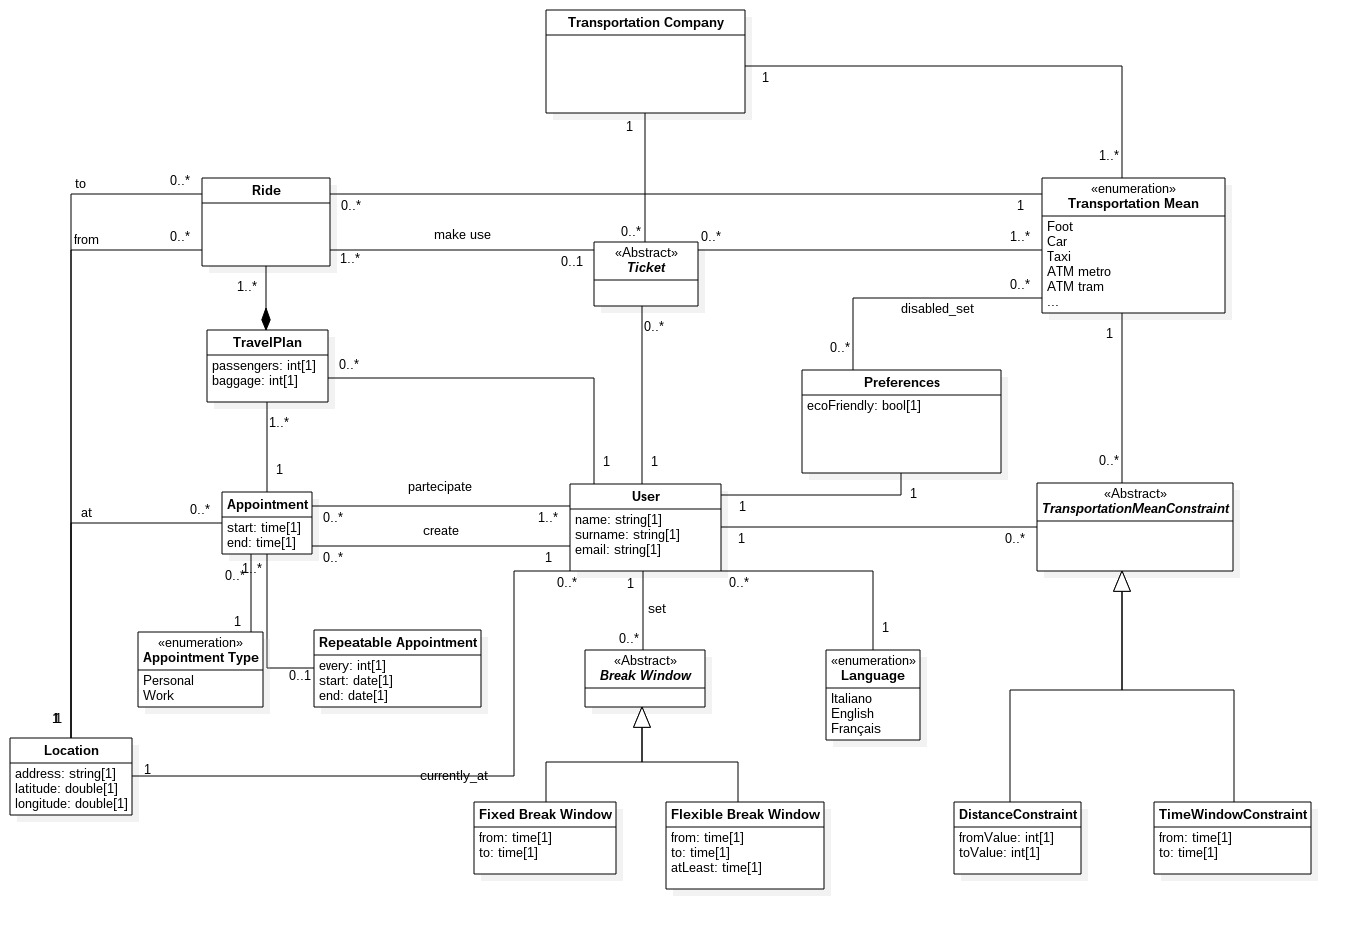
\includegraphics[width=\paperwidth-1]{Images/ClassDiagram}}
			\caption{General class diagram}
		\end{figure}
	\subsubsection{Activity diagrams}
		\begin{figure}[H]
			\centerline{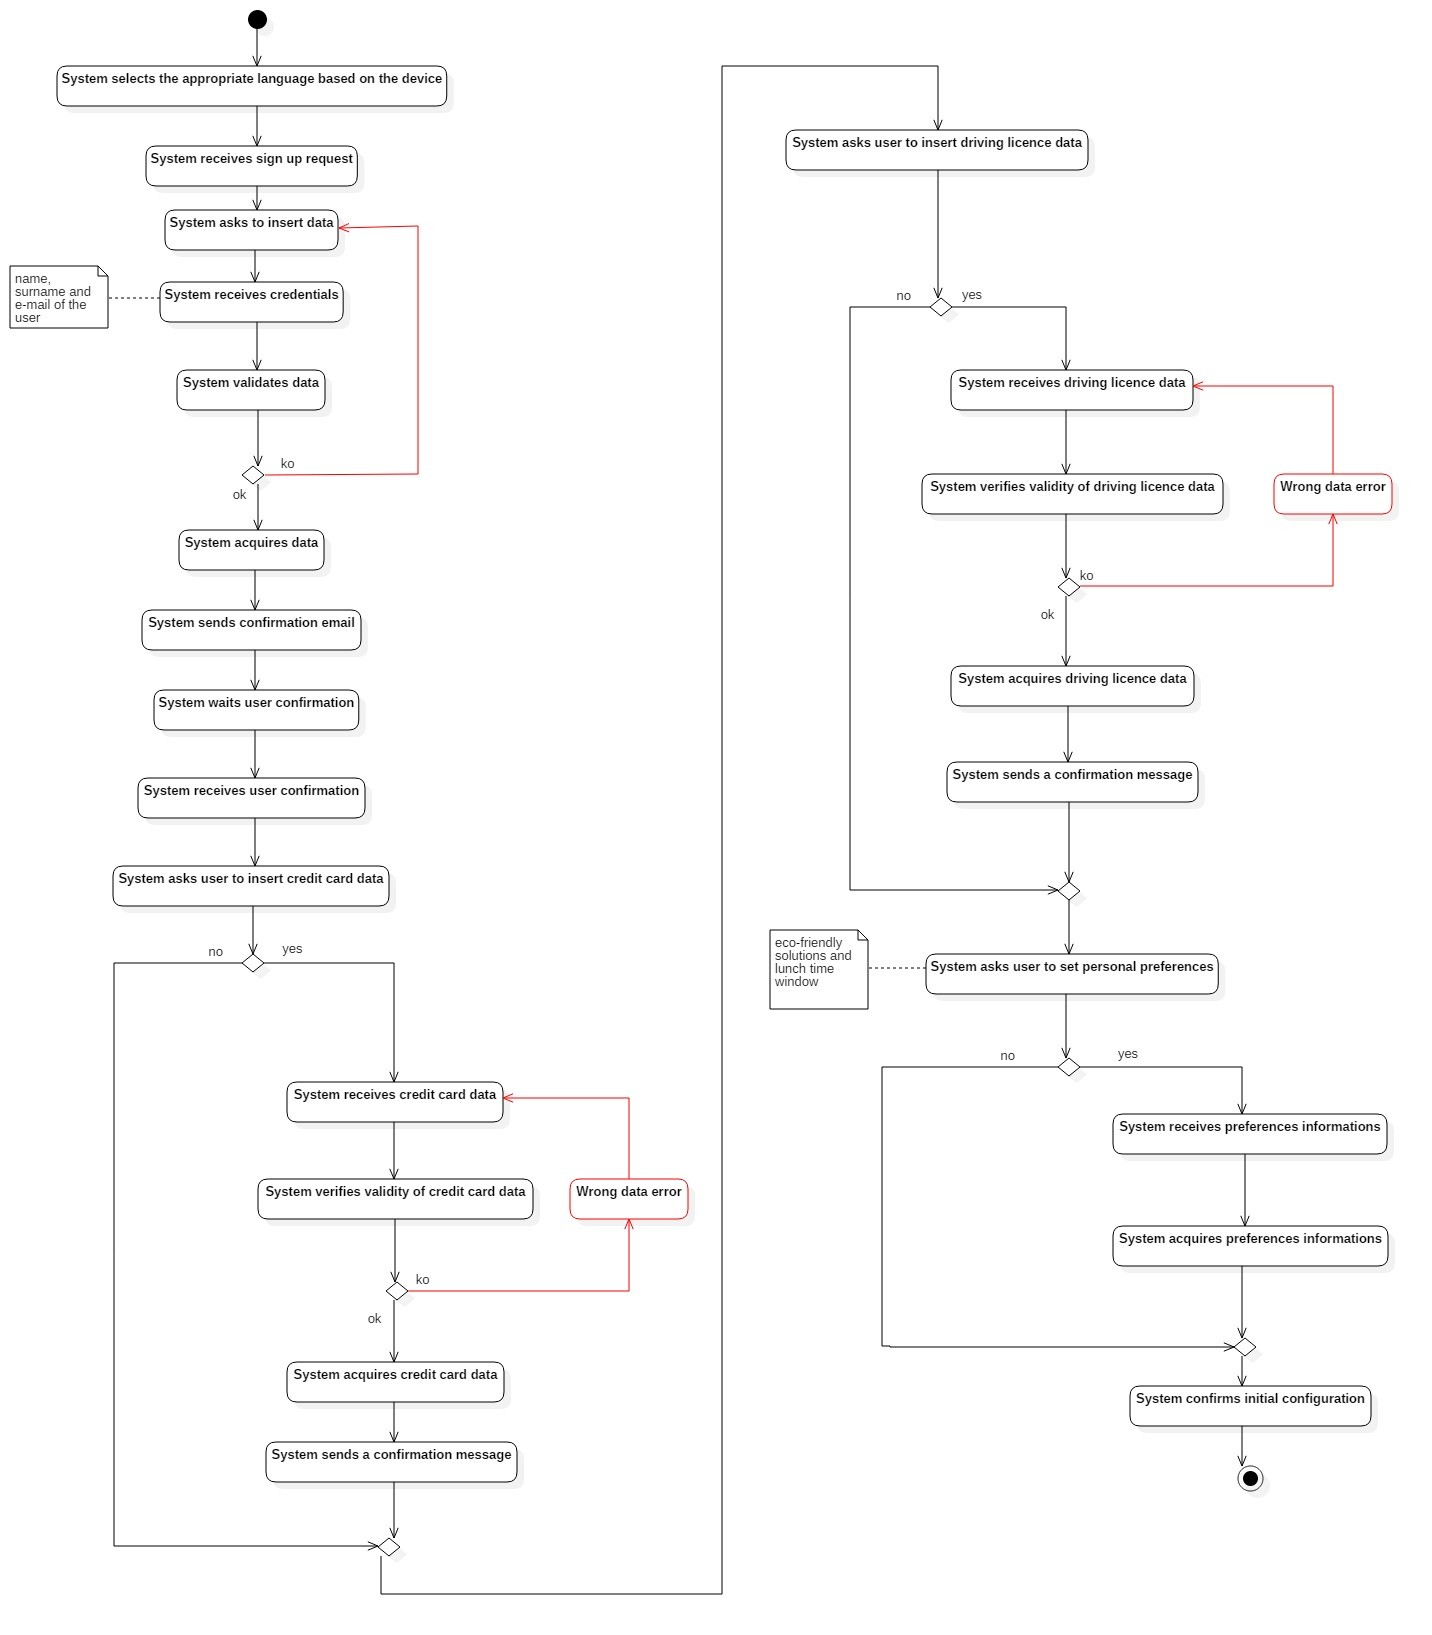
\includegraphics[height=0.75\paperheight]{Images/RegistrationDiagram}}
			\caption{Registration diagram}
		\end{figure}

%		\begin{figure}[H]
%			\centerline{\includegraphics[width=\paperwidth-1]{Images/AppointmentCreationDiagram}}
%			\caption{Appointment creation diagram}
%		\end{figure}
\subsection{Functional Requirements}
\subsection{Performance Requirements}
\subsection{Design Constraints}
	\subsubsection{Standard compliance}
	\subsubsection{Hardware limitations}
	\subsubsection{Any other constraint}
\subsection{Software System Attributes} 
	\subsubsection{Reliability}
	\subsubsection{Availability}
	\subsubsection{Security}
	\subsubsection{Maintainability}
	\subsubsection{Portability}

%------------------------------------------------------------------------------------------------------------------------------------------------
\clearpage
\section{Formal Analysis Using Alloy}
\label{sect:alloy}
\subsection{Alloy Code}
\alloyfile{../alloy.als}
\subsection{Results of Alloy Analysis}
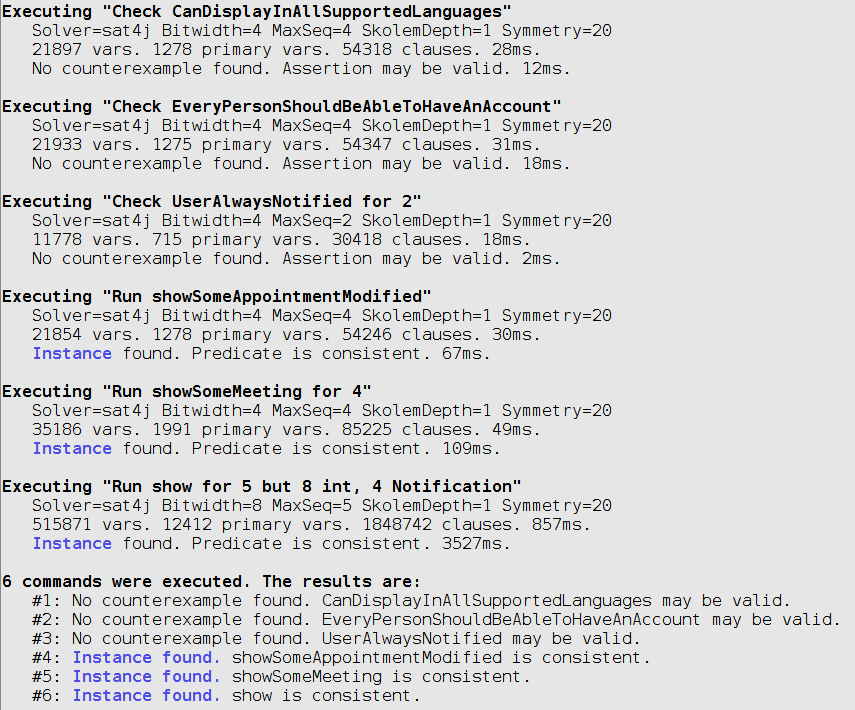
\includegraphics[scale=0.5]{Images/alloyRun}
\subsection{Alloy Model}
% TODO

%------------------------------------------------------------------------------------------------------------------------------------------------
\clearpage
\section{Effort Spent}
\label{sect:effort}
\input{sections/effort}

%------------------------------------------------------------------------------------------------------------------------------------------------
\clearpage
\section{References}
\label{sect:references}
\subsection{Software and Tools}
	\begin{itemize}
	\item
		\underline{\LaTeX\ } for typesetting document
	\item
		\underline{TeXstudio} as \LaTeX\ IDE
	\item
		\underline{GitHub} and \underline{git} for version control and team work
	\item
		\underline{StarUML} for UX diagrams
	\item
		\href{https://draw.io}{\underline{Draw.io}} for UML diagrams
	\item
		\underline{Microsoft Visio} for ER diagram
	\item
		\underline{Adobe Photoshop} for Mockups
	\end{itemize}
\subsection{Reference Documents}
	\begin{itemize}
		\item 1016-2009 - IEEE Standard for Information Technology -- Systems Design -- Software Design Descriptions: \href{http://ieeexplore.ieee.org/document/5167255/}{http://ieeexplore.ieee.org/document/5167255/}

		\item 42010-2011 - ISO/IEC/IEEE Systems and software engineering -- Architecture description:
		\\%leave here the break the line: problem with the url visualization
		 \href{http://ieeexplore.ieee.org/document/6129467/}{http://ieeexplore.ieee.org/document/6129467/}
	\end{itemize}


\end{document}